%%%%\%%%%%%%%%%%%%%%%%%%%%%%%%%%%%%%%%%%%%%%%%%%
%% Introduction aux Systèmes d'exploitation  %%
%%   * Historique                            %%
%%   * Principes fondamentaux                %%
%%   * Grandes classes de systèmes           %%
%%%%%%%%%%%%%%%%%%%%%%%%%%%%%%%%%%%%%%%%%%%%%%%

\title{Systèmes d'exploitation, 2ème année}
\subtitle{Fichiers et processus}

\author{Yves \textsc{Stadler}}\institute{Université Paul Verlaine - Metz}

\date{\today}

\begin{document}


%%
% Page de Titre
%%
\begin{frame}
\titlepage
\end{frame}

\def\sectitle{Agenda}
\section{\sectitle}
\def\subsectitle{Plan du chapitre}
\subsection{\subsectitle}

\begin{frame}{\sectitle}
\begin{block}{\subsectitle}
\begin{itemize}
\item Deadlocks
\item Famine
\item Stratégie de prévention
\end{itemize}
\end{block}
\end{frame}


\def\sectitle{Deadlock}
\section{\sectitle}
\begin{frame}{\sectitle}

\def\subsectitle{Illustration d'un deadlock}
\subsection{\subsectitle}

\begin{alertblock}{\subsectitle}
\begin{itemize}
\item On dispose de 200KB de mémoire
\item Le processus A requiert 80KB de mémoire
\item Le processus B requiert 70KB de mémoire
\item Le processus A requiert 60KB de mémoire
\item Le processus B requiert 80KB de mémoire
\end{itemize}
\end{alertblock}

\def\subsectitle{Pourquoi arrive-t-on là?}
\subsection{\subsectitle}
\begin{block}{\subsectitle}
\begin{itemize}
    \item Indépendamment chaque processus peut s'exécuter
    \item L'ordonnancement peut mener à un point ou chaque processus réserve une
    partie de la mémoire sans pour autant pouvoir entrer en section critique.
\end{itemize}
\end{block}

\end{frame}


\def\sectitle{Exemple avec deux sémaphores}
\section{\sectitle}
\begin{frame}[containsverbatim]{\sectitle}

\begin{columns}[t]
\column{.5\textwidth}
\def\subsectitle{Programme 1}
\subsection{\subsectitle}
\begin{exampleblock}{\subsectitle}
\begin{verbatim}
P(semA)
P(semB)
Critical Section
V(semB)
V(semA)
\end{verbatim}
\end{exampleblock}

\def\subsectitle{Philosophes}
\subsection{\subsectitle}
\begin{exampleblock}{\subsectitle}
\begin{verbatim}
think()
P(fork[i])
P(fork[i+1])
eat()
V(fork[i])
V(fork[i+1])
\end{verbatim}
\end{exampleblock}

\column{.5\textwidth}
\def\subsectitle{Programme 2}
\subsection{\subsectitle}
\begin{exampleblock}{\subsectitle}
\begin{verbatim}
P(semA)
P(semB)
Critical Section
V(semB)
V(semA)
\end{verbatim}
\end{exampleblock}

\end{columns}
\end{frame}



\def\sectitle{Existence d'un deadlock}
\section{\sectitle}
\begin{frame}{\sectitle}
\def\subsectitle{Coffman conditions}
\subsection{\subsectitle}
\begin{block}{\subsectitle}
\begin{itemize}
    \item Exclusion mutuelle: un seul processus à la fois peut utiliser une
    ressource
    \item Rétention: un processus conserve une ressource tout en demandant une
    autre déjà allouée
    \item Pas de préemption (de ressource)
    \item Attente circulaire: il faut une chaîne de processus dans laquelle
    chaque processus détient la ressource nécessaire au processus suivant dans
    la chaîne.
\end{itemize}
\end{block}
\end{frame}

\def\sectitle{Stratégie pour éviter l'interblocage}
\section{\sectitle}
\begin{frame}{\sectitle}
\begin{block}{\subsectitle}
\begin{itemize}
    \item S'assurer que le système n'y entre jamais
    \item Permettre au système de se bloquer et l'en sortir
    \item Ne pas s'en occuper et espérer que ça n'arrive jamais.
\end{itemize}
\end{block}
\end{frame}

\def\sectitle{Prévention}
\section{\sectitle}
\begin{frame}{\sectitle}
\def\subsectitle{Objectif}

\begin{alertblock}{\subsectitle}
\begin{itemize}
    \item Éliminer l'une des conditions de Coffman
\end{itemize}
\end{alertblock}


\subsection{\subsectitle}
\begin{block}{\subsectitle}
\begin{itemize}
    \item Éviter de mettre des exclusions lorsqu'elle ne sont pas nécessaires
    (fichiers en lecture seule).
    \item Obliger les processus à réclamer toutes leurs ressources en une fois
    (risque de famine)
    \item Refuser la rétention (si une ressource est refusée, on relâche tout)
    \item Définir un ordre dans l'attribution de ressources (peut-être moins
    efficace)
    \item Ne démarrer un processus que si on peut réserver d'avance ses
    ressources
    \item Ne donner les ressources que si le système reste dans un état sain.
    \item Détection facile, prévention difficile.
\end{itemize}
\end{block}
\end{frame}


\def\sectitle{Algorithme du Banquier}
\section{\sectitle}
\begin{frame}{\sectitle}
\def\subsectitle{Conditions}
\subsection{\subsectitle}
\begin{block}{\subsectitle}
\begin{itemize}
    \item Un état est sur lorsqu'il existe une séquence sûre pour tous les
    processus
    \item Une séquence de processus $P_{i}$ est sûre si $\forall P_{i}$ les
    ressources que ce processus n'a pas réclamé peuvent être satisfaites ou sont
    alloué aux processus le précédent dans la séquence.
\end{itemize}
\end{block}
\end{frame}

\def\sectitle{Algorithme du Banquier}
\section{\sectitle}
\begin{frame}{\sectitle}
\def\subsectitle{Réalisation}
\subsection{\subsectitle}
\begin{block}{\subsectitle}
\begin{itemize}
    \item Quand un processus arrive, il indique la quantité maximale de chaque
    ressource qu'il compte utilisée.
    \item Quand un processus se voit allouer des ressources, il doit les
    restituer dans un délai de temps fini.
\end{itemize}
\end{block}
\def\subsectitle{Implémentation}
\subsection{\subsectitle}
\begin{block}{\subsectitle}
\begin{itemize}
    \item Quantité de ressources potentielles a allouer (MAX)
    \item Quantité de ressources déjà alloués (CUR)
    \item Quantité de ressources dont le système dispose (AVL)
    \item Optionnellement la quantité de ressources potentiellement requise (NED).
\end{itemize}
\end{block}
\end{frame}

\begin{frame}{\sectitle}
\def\subsectitle{Allocations}
\subsection{\subsectitle}
\begin{block}{\subsectitle}
\begin{itemize}
    \item Requête <= max; Sinon le programme à mentit, exception;
    \item Requête <= disponible; Sinon attente.
    \item NED = MAX - CUR.
\end{itemize}
\end{block}

\def\subsectitle{Vérfications}
\subsection{\subsectitle}
\begin{block}{\subsectitle}
\begin{itemize}
    \item Est-il possible d'allouer NED pour au moins un processus 
    \item Permet de faire terminer ce processus
    \item Libère les ressources
    \item Si impossible, état "unsafe". 
\end{itemize}
\end{block} 
\end{frame}

\begin{frame}[containsverbatim]{\sectitle}
\def\subsectitle{Exemple}
\subsection{\subsectitle}
\begin{exampleblock}{\subsectitle}
\begin{verbatim}
MAX A B C    AVL A B C    CUR A B C    NED A B C
P1  5 7 2    ALL 6 9 2    P1  0 0 0    P1  5 7 2
P2  3 5 1                 P1  0 0 0    P2  3 5 1
\end{verbatim}
\end{exampleblock}

\begin{exampleblock}{\subsectitle}
\begin{verbatim}
MAX A B C    AVL A B C    CUR A B C    NED A B C
P1  5 7 2    ALL 1 9 2    P1  5 0 0    P1  0 7 2
P2  3 5 1                 P1  0 0 0    P2  3 5 1
\end{verbatim}
\end{exampleblock}

\end{frame}



\def\sectitle{Représentation graphique}
\section{\sectitle}
\begin{frame}{\sectitle}
\def\subsectitle{Définitions}
\subsection{\subsectitle}
\begin{block}{\subsectitle}
\begin{itemize}
    \item Deux types de n{\oe}uds: processus ou ressources
    \item Une arrête d'un processus à une ressource est une demande
    \item Une arrête d'une ressource à un processus est une allocation
    \item L'objectif est de découvrir les cycles
\end{itemize}
\end{block}

\begin{figure}
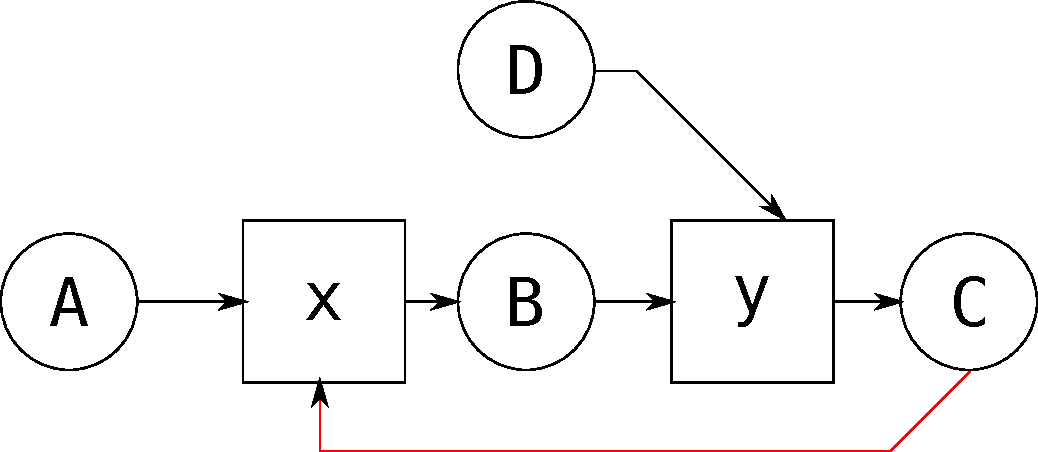
\includegraphics[width=.8\textwidth]{images/deadlockGraph01.pdf}
\end{figure}

\end{frame}

\begin{frame}{\sectitle}
\begin{block}{\subsectitle}
\def\subsectitle{Détections des cycles}
\subsection{\subsectitle}
\begin{itemize}
    \item Soit $D_{T}$ l'ensemble des processus sur lesquels D attend.
    \item $D_{T} = T$ si T ne veut rien.
    \item $D_{T} = D_{owner(R)}$
\end{itemize}
\end{block}

\begin{exampleblock}{\subsectitle}
\begin{itemize}
    \item $D_{C} = {C}$
    \item $D_{D} = {C,D}$
    \item $D_{B} = {C,B}$
    \item $D_{A} = {B,C,A}$
    \item C voulant x détecte un cycle dans $D_{B}$
\end{itemize}
\end{exampleblock}

\end{frame}


\def\sectitle{Sémaphores}
\section{\sectitle}
\begin{frame}[containsverbatim]{\sectitle}
\def\subsectitle{Headers}
\subsection{\subsectitle}
\begin{block}{\subsectitle}
\begin{verbatim}
#include <sys/types.h>
#include <sys/ipc.h>
#include <sys/sem.h>
\end{verbatim}
\end{block}
\def\subsectitle{Fonctions de création}
\subsection{\subsectitle}
\begin{block}{\subsectitle}
\begin{verbatim}
int semget(key_t key, int nsems, int semflg);
\end{verbatim}
\begin{itemize}
    \item Appel et renvoi \texttt{nsems} sémaphores \texttt{key}
    \item \texttt{semflg : IPC\_PRIVATE | IPC\_CREAT}
    \item Le flag permet aussi de choisir les permissions du sémaphore.
\end{itemize}
\end{block}

\end{frame}

\def\sectitle{Structure pour opération sur sémaphores}
\section{\sectitle}
\begin{frame}[containsverbatim]{\sectitle}
\def\subsectitle{Fonction de contrôle}
\subsection{\subsectitle}
\begin{block}{\subsectitle}
\begin{verbatim}
int semctl(int semid, int semnum, int cmd, ...);
union semun {
    int              val;  /* Value for SETVAL */
    struct semid_ds *buf;  /* Buffer for IPC_STAT, IPC_SET */
    unsigned short  *array;/* Array for GETALL, SETALL */
    struct seminfo  *__buf;/* Buffer for IPC_INFO
                                (Linux specific) */
};
\end{verbatim}
\begin{itemize}
    \item Opération \texttt{cmd: IPC\_STAT | IPC\_SET | IPC\_RMID}
    \item Le quatrième paramètre quand il existe est la structure \texttt{semun}
\end{itemize}
\end{block}
\end{frame}

\begin{frame}[containsverbatim]{\sectitle}
\def\subsectitle{Fonction d'usage}
\subsection{\subsectitle}
\begin{block}{\subsectitle}
\begin{verbatim}
int semop(int semid, struct sembuf *sops, unsigned nsops);

unsigned short sem_num;  /* semaphore number */
short          sem_op;   /* semaphore operation */
short          sem_flg;  /* operation flags */
\end{verbatim}
\begin{itemize}
    \item Opérations sur \texttt{sem\_num}
    \item de type \texttt{sem\_op} (entier, incr/décrémente le sémaphore de
    cette valeur
    \item avec un flag \texttt{sem\_flg : IPC\_NOWAIT | SEM\_UNDO} 
\end{itemize}
\end{block}
\end{frame}

\def\sectitle{Les primitives exec}
\section{\sectitle}
\begin{frame}{\sectitle}
\begin{block}{\subsectitle}
\begin{itemize}
    \item On connait le nombre d'arguments : famille \texttt{execl}
    \item On ne connait pas le nombre d'arguments : famille \texttt{execv}
\end{itemize}
\end{block}

\begin{block}{\subsectitle}
\begin{itemize}
    \item Remplace l'image du programme par un autre
    \item Toutes les instructions qui suivent exec ne seront jamais exécutée.
\end{itemize}
\end{block}

\end{frame}


\end{document}
